\section{Grafici ed immagini}
\begin{figure}[h]
	\centering
	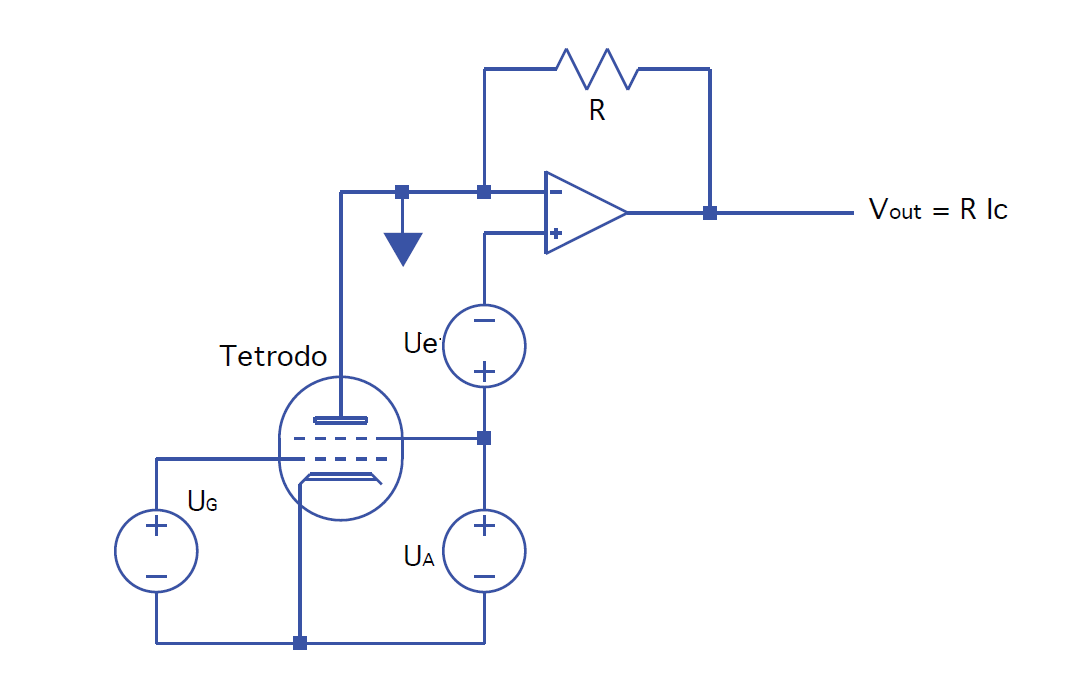
\includegraphics[scale=0.5]{apparato.png}
	\caption{Schema dell'apparato utilizzato nell'esperienza}
	\label{f:apparato}
\end{figure}

\begin{figure}[h]
	\centering
	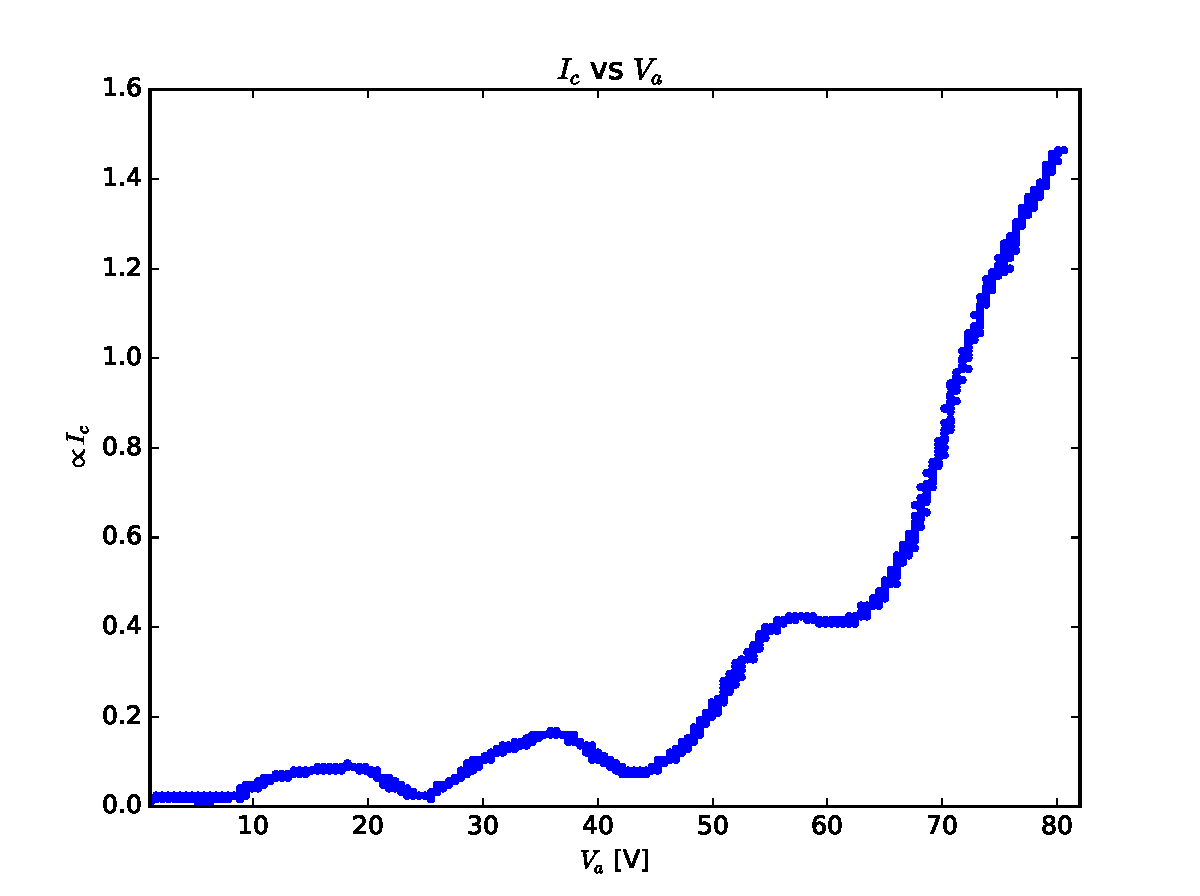
\includegraphics[scale=0.5]{figure_1.pdf}
	\caption{grafico di $I_c$ in funzione di $U_a$}
	\label{f:figura_1}
\end{figure}

\begin{figure}[h]
	\centering
	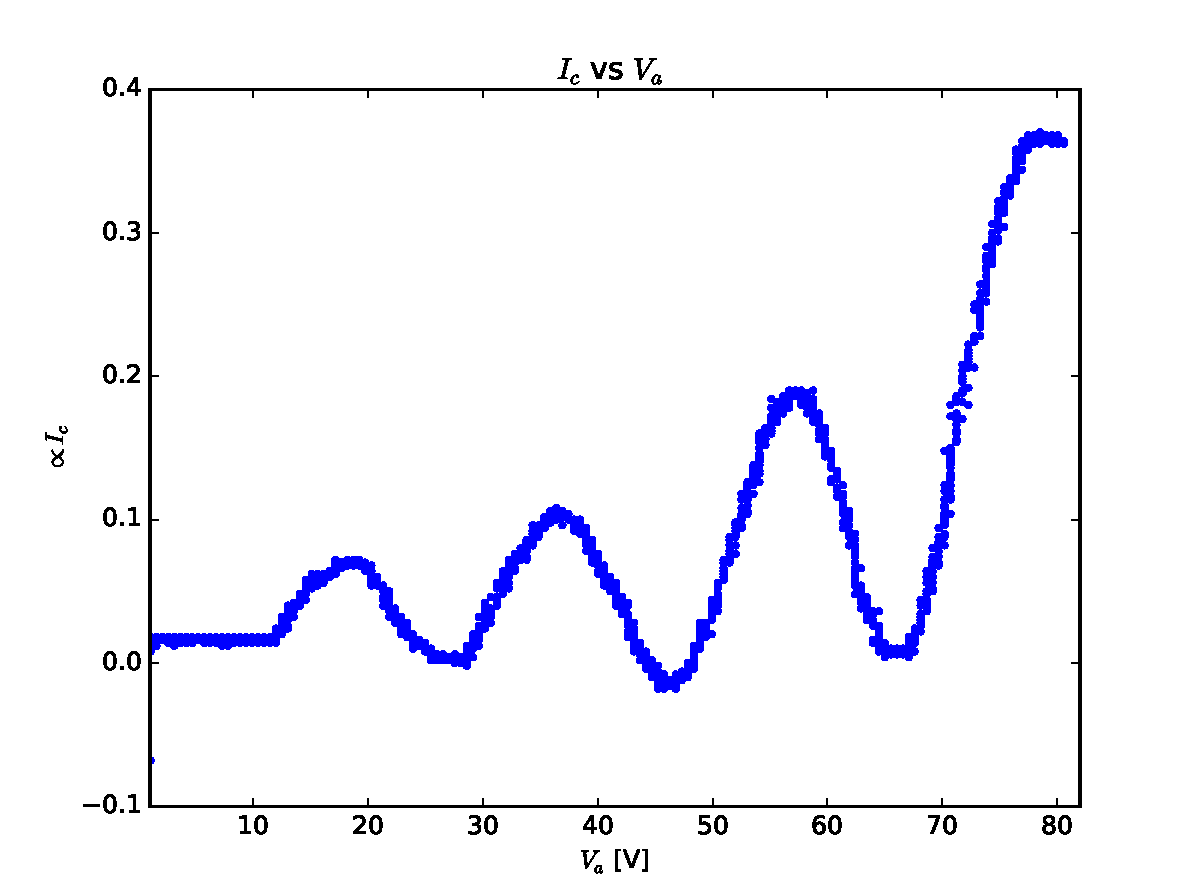
\includegraphics[scale=0.5]{figure_3.pdf}
	\caption{grafico di $I_c$ in funzione di $U_a$}
	\label{f:figura_3}
\end{figure}

\begin{figure}[h]
	\centering
	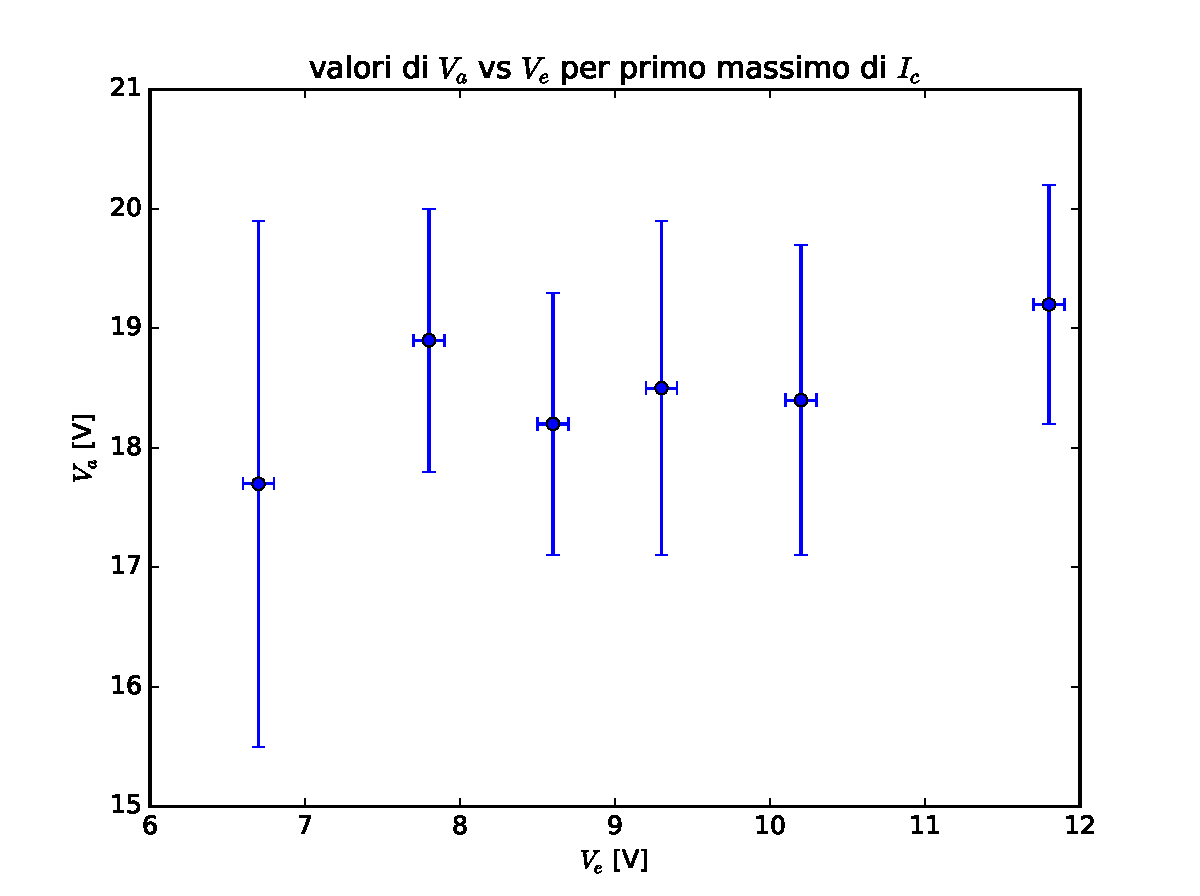
\includegraphics[scale=0.5]{figure_0.pdf}
	\caption{valori di $U_a$ al variare di $U_E$ in corrispondenza del primo massimo di $I_c$  }
	\label{f:figura_0}
\end{figure}

\begin{figure}[h]
	\centering
	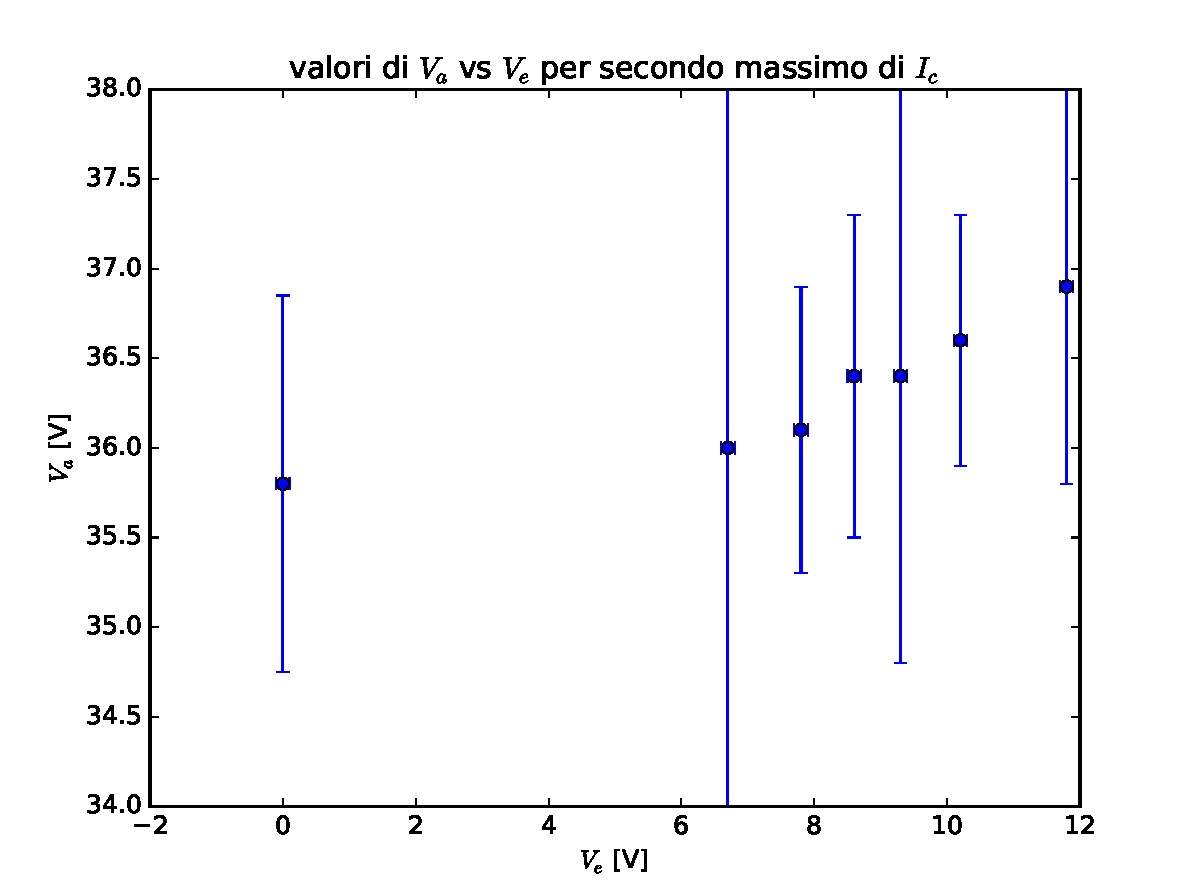
\includegraphics[scale=0.5]{figure_2.pdf}
	\caption{valori di $U_a$ al variare di $U_E$ in corrispondenza del secondo massimo di $I_c$  }
	\label{f:figura_2}
\end{figure}

\begin{figure}[h]
	\centering
	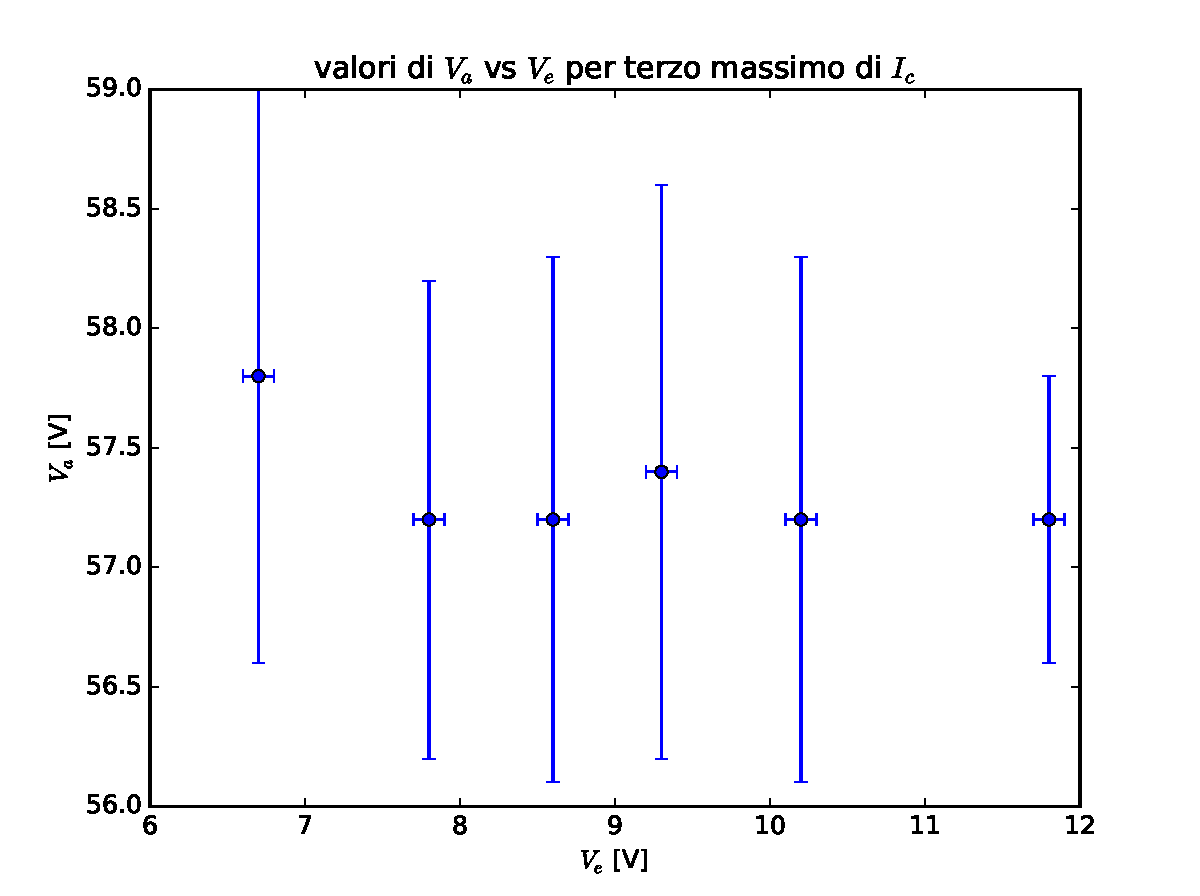
\includegraphics[scale=0.5]{figure_4.pdf}
	\caption{valori di $U_a$ al variare di $U_E$ in corrispondenza del terzo massimo di $I_c$  }
	\label{f:figura_4}
\end{figure}

\begin{figure}[h]
	\centering
	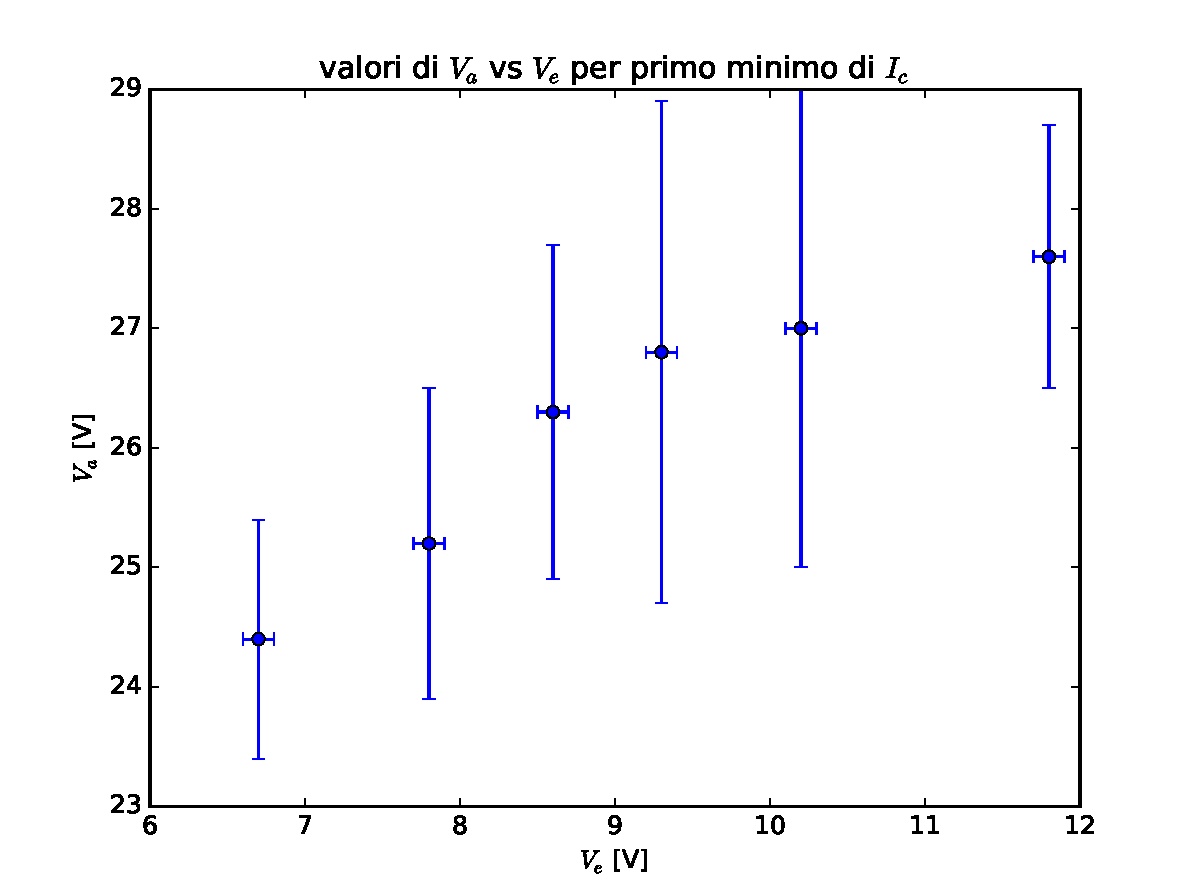
\includegraphics[scale=0.5]{figure_6.pdf}
	\caption{valori di $U_a$ al variare di $U_E$ in corrispondenza del primo minimo di $I_c$  }
	\label{f:figura_6}
\end{figure}

\begin{figure}[h]
	\centering
	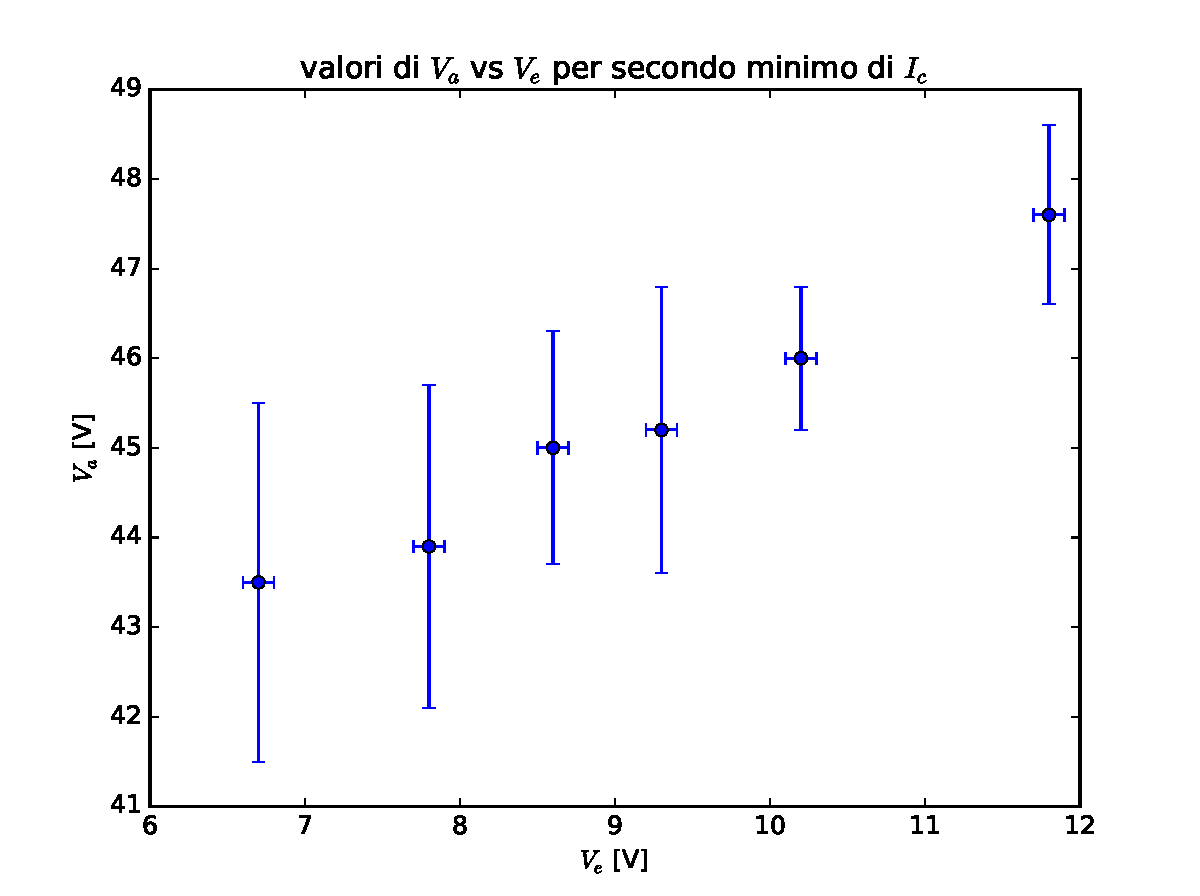
\includegraphics[scale=0.5]{figure_8.pdf}
	\caption{valori di $U_a$ al variare di $U_E$ in corrispondenza del secondo minimo di $I_c$  }
	\label{f:figura_8}
\end{figure}

\begin{figure}[h]
	\centering
	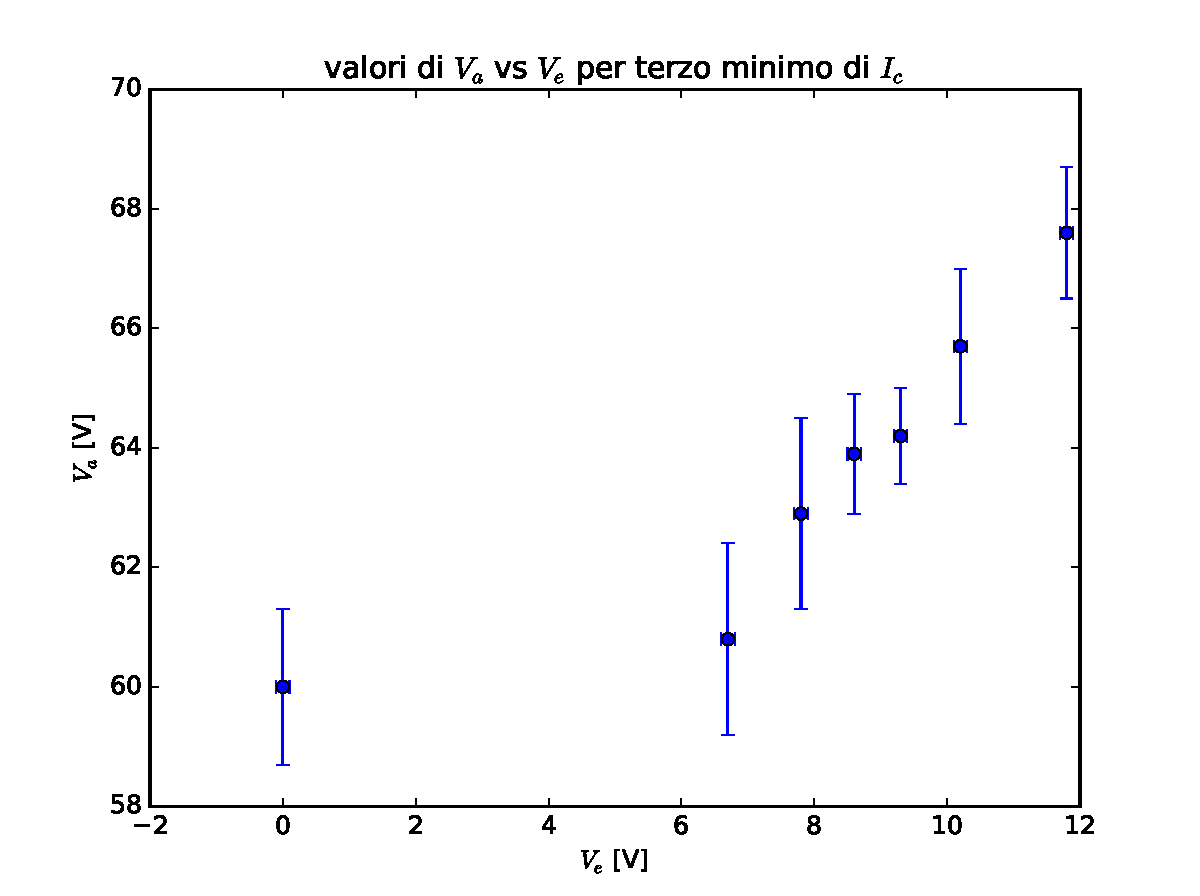
\includegraphics[scale=0.5]{figure_10.pdf}
	\caption{valori di $U_a$ al variare di $U_E$ in corrispondenza del terzo minimo di $I_c$  }
	\label{f:figura_10}
\end{figure}